\documentclass[a5paper,10pt]{article}
 
\usepackage{extsizes}
\usepackage{cmap}
\usepackage[T2A]{fontenc}
\usepackage[utf8x]{inputenc}
\usepackage[english, russian]{babel}

\usepackage{misccorr}

%%%%%%%%%%%%%%%%%%%%%%%%%%%%%%%%%%%%%%%%%%%%%%%%%%%%%%%%%%%%%%%%%%%%%%%%%%%%%%%%%%  
\usepackage{graphicx} % для вставки картинок
\graphicspath{{img/}}
\usepackage{amssymb,amsfonts,amsmath,amsthm} % математические дополнения от АМС

% \usepackage{fontspec}
% \usepackage{unicode-math}

\usepackage{indentfirst} % отделять первую строку раздела абзацным отступом тоже
\usepackage[usenames,dvipsnames]{color} % названия цветов
\usepackage{makecell}
\usepackage{multirow} % улучшенное форматирование таблиц
\usepackage{ulem} % подчеркивания
\linespread{1.3} % полуторный интервал
% \renewcommand{\rmdefault}{ftm} % Times New Roman (не работает)
\frenchspacing
\usepackage{geometry}
\geometry{left=1cm,right=1cm,top=2cm,bottom=1cm,bindingoffset=0cm}
\usepackage{titlesec}
\usepackage{float}
% \definecolor{black}{rgb}{0,0,0}
% \usepackage[colorlinks, unicode, pagecolor=black]{hyperref}
% \usepackage[unicode]{hyperref} %ссылки
\usepackage{fancyhdr} %загрузим пакет
\pagestyle{fancy} %применим колонтитул
\fancyhead{} %очистим хидер на всякий случай
\fancyhead[R]{Сарафанов Ф.Г.} %номер страницы слева сверху на четных и справа на нечетных
\fancyhead[C]{Механика}
\fancyhead[L]{Иродов 1.242} 
\fancyfoot{} %футер будет пустой
% \fancyfoot[CO,CE]{\thepage}
\renewcommand{\labelenumii}{\theenumii)}


\usepackage{tikz}
\usetikzlibrary{scopes}
\usetikzlibrary{%
	 decorations.pathreplacing,%
	 decorations.pathmorphing,%
	patterns,%
	calc,%
	scopes,%
	arrows,%
	through,%
	% arrows.spaced,%
}
\newcommand{\vangle}{\mathop{\mathstrut^\wedge}\nolimits}
\newcommand{\average}[1]{\langle{#1}\rangle}
\usepackage{wrapfig}
\newcommand{\RN}[1]{%
  \textup{\tiny\uppercase\expandafter{\romannumeral#1}}%
}
\begin{document}

\begin{figure}[H]
	\centering
\begin{tikzpicture}[
	force/.style={>=latex,draw=blue,fill=blue},
	acceleration/.style={>=open triangle 60,draw=blue,fill=blue},
	% axis/.style={densely dashed,gray,font=\small},
	axis/.style={densely dashed,black!60,font=\small},
	M/.style={rectangle,draw,fill=lightgray,minimum size=0.5cm,thin},
	m2/.style={draw=black!30, rectangle,draw,thin, fill=blue!2, minimum width=0.7cm,minimum height=0.7cm},
	m1/.style={draw=black!30, rectangle,draw,thin, fill=blue!2, minimum width=0.7cm,minimum height=0.7cm},
	plane/.style={draw=black!30, very thick, fill=blue!5, line width=1pt},
	% base/.style={draw=black!70, very thick, fill=blue!4, line width=2pt},
	string/.style={draw=black, thick},
	pulley/.style={thick},
	interface1/.style={draw=gray!60,
		% The border decoration is a path replacing decorator. 
		% For the interface style we want to draw the original path.
		% The postaction option is therefore used to ensure that the
		% border decoration is drawn *after* the original path.
		postaction={draw=gray!60,decorate,decoration={border,angle=-135,
					amplitude=0.3cm,segment length=2mm}}},
	interface/.style={
		pattern = north east lines,
		draw    = none,
		pattern color=gray!60,          
	},
	plank/.style={
		fill=black!60, 
		draw=black,
		minimum width=3cm,
		inner ysep=0.1cm,
		outer sep=0pt,
		yshift=0.75cm,
		pattern = north east lines,
		pattern color=gray!60, 
	},
	cargo/.style={
		rectangle,
		fill=black!70,              
		inner sep=2.5mm,
	}
]
    % \node {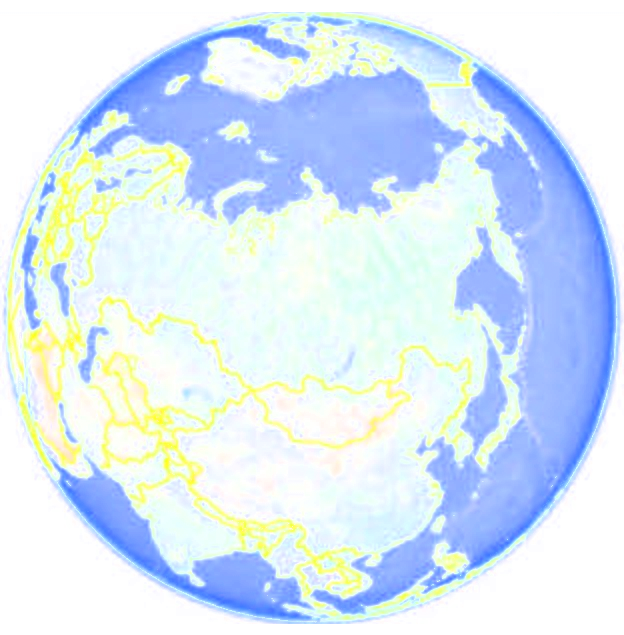
\includegraphics[scale=.092]{earth.png}};    
	\draw[fill=black!10] (0,0) circle(1cm);
	\draw[axis] (0,0) circle(2cm);
	\node[left] at (-2.1,0) {Запад};
	\node[left] at (3.4,0) {Восток};
	\coordinate (s) at (0,2);
	\draw[fill=black] (s) circle (2pt);
	\draw[force,->] (s) -- ++(1,0) node[above] {$\vec{v}$};
	\draw[force,->] (s) -- ++(0,-0.5) node[left] {$\vec{F}_g$};
	\draw[axis,->] (s) -- (0,0);% node[below] {$\vec{N}_{2n}$};

\end{tikzpicture}
\end{figure}
Земля вращается с запада на восток. Линейная скорость неподвижной точки на экваторе $v_\text{з}$:
\begin{gather*}
	T=\frac{2\pi}{\omega}=\frac{2\pi{R}}{v_\text{з}}\\
	v_\text{з}=\frac{2\pi{R}}{T}
\end{gather*}
Тогда можно найти собственную скорость спутника $v$:
\begin{gather*}
	v'=v-v_\text{з}\\
	v'=\frac{2\pi{R}}{\tau}\\
	v=\frac{2\pi{R}}{T}+\frac{2\pi{R}}{\tau}=2\pi{R}(\frac{\tau+T}{\tau{T}})
\end{gather*}
Введем нормальную ось $n$, направленную к центру Земли.
\begin{gather*}
	v=const\Longrightarrow a=a_n=\frac{v^2}{R}=\frac{4\pi^2R}{T^2}(1+\frac{T}{\tau})^2\\
	m\vec{a}=\vec{F}_g\\
	\text{n: }ma_n=G\frac{Mm}{R^2}\\
	M=\frac{a_n\cdot{R^2}}{G}=\frac{4\pi^2R^3}{G\tau^2}(1+\frac{T}{\tau})^2=6\cdot10^{24}\text{ кг}\\
\end{gather*}
% \begin{equation*}
% 	\begin{aligned}[c]
% 		\textbf{I.  }
% 		m\vec{a}=\vec{N}_3+m\vec{g}\\
% 		\text{n: }ma_n=N_3+mg\\
% 		P_3=N_3\\
% 		P_3=ma_n-mg=\\
% 		=m(\frac{v^2}{R}-g)=700\text{\,H}
% 	\end{aligned}
% 		% \qquad\Longrightarrow\qquad
% 		\qquad\qquad
% 	\begin{aligned}[c]
% 	\textbf{II.  }
% 	m\vec{a}=\vec{N}_2+m\vec{g}\\
% 	\text{n: }ma_n=N_{2n}\\
% 	\text{$\tau$: }mg=N_{2\tau}\\
% 	P_2=N_2=\sqrt{N_{2n}^2+N_{2\tau}^2}=\\
% 	m\sqrt{\frac{v^4}{R^2}+g^2}=1565\text{\,H}
% 	\end{aligned}
% \end{equation*}

\end{document}